%Не забыть:
%--------------------------------------
%Вставить колонтитулы, поменять название на титульнике



%--------------------------------------

\documentclass[a4paper, 12pt]{article} 

%--------------------------------------
%Russian-specific packages
%--------------------------------------
%\usepackage[warn]{mathtext}
\usepackage[T2A]{fontenc}
\usepackage[utf8]{inputenc}
\usepackage[english,russian]{babel}
\usepackage[intlimits]{amsmath}
\usepackage{esint}
%--------------------------------------
%Hyphenation rules
%--------------------------------------
\usepackage{hyphenat}
\hyphenation{ма-те-ма-ти-ка вос-ста-нав-ли-вать}
%--------------------------------------
%Packages
%--------------------------------------
\usepackage{amsmath}
\usepackage{amssymb}
\usepackage{amsfonts}
\usepackage{amsthm}
\usepackage{latexsym}
\usepackage{mathtools}
\usepackage{epstopdf}
\usepackage{etoolbox}%Булевые операторы
\usepackage{extsizes}%Выставление произвольного шрифта в \documentclass
\usepackage{geometry}%Разметка листа
\usepackage{indentfirst}
\usepackage{wrapfig}%Создание обтекаемых текстом объектов
\usepackage{fancyhdr}%Создание колонтитулов
\usepackage{setspace}%Настройка интерлиньяжа
\usepackage{lastpage}%Вывод номера последней страницы в документе, \lastpage
\usepackage{soul}%Изменение параметров начертания
\usepackage{hyperref}%Две строчки с настройкой гиперссылок внутри получаеммого
\usepackage[usenames,dvipsnames,svgnames,table,rgb]{xcolor}% pdf-документа
\usepackage{multicol}%Позволяет писать текст в несколько колонок
\usepackage{cite}%Работа с библиографией
\usepackage{subfigure}% Человеческая вставка нескольких картинок
\usepackage{tikz}%Рисование рисунков
\usepackage{float}
% Для картинок Моти
\usepackage{misccorr}
\usepackage{lscape}
\usepackage{cmap}


\usepackage{graphicx,xcolor}
\graphicspath{{Pictures/}}
\DeclareGraphicsExtensions{.pdf,.png,.jpg}

%----------------------------------------
%Список окружений
%----------------------------------------
\newenvironment {theor}[2]
{\smallskip \par \textbf{#1.} \textit{#2}  \par $\blacktriangleleft$}
{\flushright{$\blacktriangleright$} \medskip \par} %лемма/теорема с доказательством
\newenvironment {proofn}
{\par $\blacktriangleleft$}
{$\blacktriangleright$ \par} %доказательство
%----------------------------------------
%Список команд
%----------------------------------------



\newcommand{\grad}
{\mathop{\mathrm{grad}}\nolimits} %градиент

\newcommand{\diver}
{\mathop{\mathrm{div}}\nolimits} %дивергенция

\newcommand{\Def}[1]
{\underline{\textbf{#1}}} %определение

\newcommand{\RN}[1]
{\MakeUppercase{\romannumeral #1}} %римские цифры

\newcommand {\theornp}[2]
{\textbf{#1.} \textit{ #2} \par} %Написание леммы/теоремы без доказательства

\newcommand{\qrq}
{\ensuremath{\quad \Rightarrow \quad}} %Человеческий знак следствия

\newcommand{\qlrq}
{\ensuremath{\quad \Leftrightarrow \quad}} %Человеческий знак равносильности

\renewcommand{\phi}{\varphi} %Нормальный знак фи

\newcommand{\me}
{\ensuremath{\mathbb{E}}}

\newcommand{\md}
{\ensuremath{\mathbb{D}}}



%\renewcommand{\vec}{\overline}




%----------------------------------------
%Разметка листа
%----------------------------------------
\geometry{top = 3cm}
\geometry{bottom = 2cm}
\geometry{left = 0.7cm}
\geometry{right = 0.7cm}
%----------------------------------------
%Колонтитулы
%----------------------------------------
\pagestyle{fancy}%Создание колонтитулов
\fancyhead{}
%\fancyfoot{}
\fancyhead[C]{\textsc{Фотонные кристаллы}}%Вставить колонтитул сюда
%----------------------------------------
%Интерлиньяж (расстояния между строчками)
%----------------------------------------
%\onehalfspacing -- интерлиньяж 1.5
%\doublespacing -- интерлиньяж 2
%----------------------------------------
%Настройка гиперссылок
%----------------------------------------
\hypersetup{				% Гиперссылки
	unicode=true,           % русские буквы в раздела PDF
	pdftitle={Заголовок},   % Заголовок
	pdfauthor={Автор},      % Автор
	pdfsubject={Тема},      % Тема
	pdfcreator={Создатель}, % Создатель
	pdfproducer={Производитель}, % Производитель
	pdfkeywords={keyword1} {key2} {key3}, % Ключевые слова
	colorlinks=true,       	% false: ссылки в рамках; true: цветные ссылки
	linkcolor=blue,          % внутренние ссылки
	citecolor=blue,        % на библиографию
	filecolor=magenta,      % на файлы
	urlcolor=cyan           % на URL
}
%----------------------------------------
%Работа с библиографией (как бич)
%----------------------------------------
\renewcommand{\refname}{Список литературы}%Изменение названия списка литературы для article
%\renewcommand{\bibname}{Список литературы}%Изменение названия списка литературы для book и report
%----------------------------------------
\begin{document}
\begin{titlepage}
\begin{center}
\textsc{Национальный исследовательский университет "Высшая школа экономики"\\[5mm]
Факультет Физики}

\vfill

\textbf{ОТЧЁТ ПО ЛАБОРАТОРНОЙ РАБОТЕ \\[3mm]
"ФОТОННЫЕ КРИСТАЛЛЫ"\\[3mm]
по курсу "Оптика"
\\[20mm]
}
\end{center}

\hfill
\begin{minipage}{.5\textwidth}
Выполнила:\\[2mm] 
Фазлиахметова Олеся Камилевна\\
БФЗ193\\
2 курс\\[5mm]

Проверила:\\[2mm] 
Готовко С. К. 
\end{minipage}%
\vfill
\begin{center}
 Москва\\
 \today
\end{center}
\end{titlepage}



\tableofcontents

\newpage

	\section{Цель работы}


\textbf{Пункт 1: Определение минимума прохождения}
	\begin{enumerate}
\item Определите, на какой длине волны находится стоп-зона при $\theta=0$.
\item  Измерьте зависимость угла поворота образца $\theta$ от угла дифракции $\phi$.
\item  Постройте линеаризованный график $\theta(\phi)$.
\item  Из графика определите средний показатель преломления кристалла $n$ и период изменения показателя преломления $D$.
	\end{enumerate}

\textbf{Пункт 2: Зависимость интенсивности лазерного излучения от величины угла.}
	\begin{enumerate}
\item Измерьте зависимость интенсивности лазерного излучения $I$ (в $\mu A$), прошедшего через фотонный кристалл, от величины угла $\theta$.
\item Постройте график полученной зависимости.
\item Определите угол падения $\theta_0$, соответствующий минимуму пропускания на длине волны лазера.
\item Определите ширину провала $\Delta \theta_0$ на графике зависимости $I(\theta)$ на уровне половины его глубины.
\item Определите нормальную (при $\theta=0$ удовлетворяющую уравнению $2Dn=m\lambda^{(n)}$) длину волны минимума пропускания $\lambda^{(n)}$.
	\end{enumerate}

	\section{Оборудование}


\begin{enumerate}

	\item Фотонный кристалл;

	\item Дифракционная решетка;

	\item Линза;

	\item Лампа;

	\item Включатель;

	\item Оптическая скамья с транспортирами;

	\item Спектральное плечо.

\end{enumerate}

\section{Теоретическая справка}

\subsection{Фотонные кристаллы}

Фотонные кристаллы являются материалами, показатель преломления которых периодически изменяется на масштабах, сравнимых с длиной волны света. В оптическом спектре фотонных кристаллов существуют узкие области длин волн, для которых распространение света подавляется. Эти необычные оптические свойства используются для создания разнообразных оптических элементов на основе фотонных кристаллов (оптических фильтров, отражателей).
В данной работе вам предлагается изучить свойства фотонных кристаллов на примере пористы (содержащих воздушные каналы) пленок оксида алюминия. Структура образцов, полученных с помощью электрохимического окисления (анодирования) алюминия, может быть представлена как система несвязанных цилиндрических каналов, расположенных перпендикулярно поверхности образца (Рис. \ref{im:1}).


\begin{figure}[H]
	\centering
	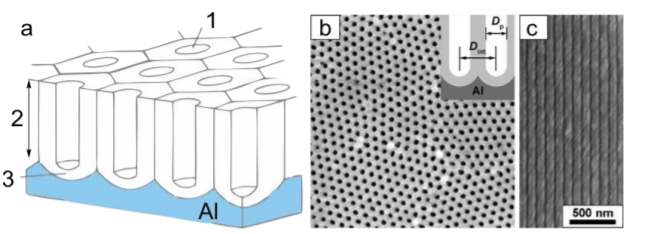
\includegraphics[scale=0.7]{1}
	\caption{ (а) Схематическая структура пористой плёнки оксида алюминия:(1)-пора, (2)-
пористый слой, (3)-барьерный слой. Изображение плёнки, полученное с помощью электронного
микроскопа: (b) вид сверху, (c) поперечное сечение}
	\label{im:1}
\end{figure}

Диаметр пор и расстояние между ними зависят от условий электрохимической обработки, позволяющей получать структуры с переменной пористостью перпендикулярно поверхности оксидной пленки, благодаря изменению напряжения во время анодирования (Рис. \ref{im:3}).

\begin{figure}[H]
	\centering
	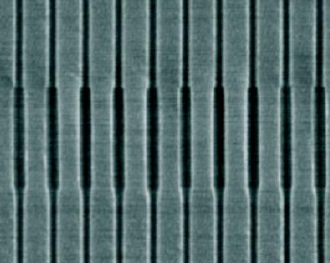
\includegraphics[scale=0.8]{3}
	\caption{Изображение поперечного разреза анодного оксида алюминия, полученное с
помощью электронного микроскопа [Nat.Mater., 2006, 5, 741]}
	\label{im:3}
\end{figure}

Изменение пористости оксидной пленки приводит к изменению её показателя преломления. Заметим, что показатель преломления исследуемых образцов периодически изменяется только в одном направлении: перпендикулярно поверхности пленки. Поэтому изучаемые образцы являются \textit{одномерными фотонными кристаллами}. Следует отметить, что тонкие плёнки анодного оксида алюминия c постоянным диаметром оптически прозрачны, тогда как фотонные кристаллы окрашены благодаря явлению интерференции света в их слоистой структуре.

\begin{figure}[H]
	\centering
	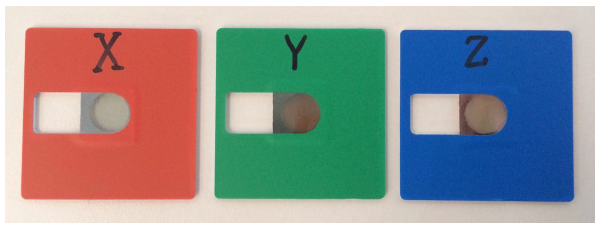
\includegraphics[scale=0.7]{4}
	\caption{Образцы фотонных кристаллов.}
	\label{im:4}
\end{figure}

\subsection{Закон Брэгга-Снелла}

Образцы фотонных кристаллов, исследуемые в данной задаче, состоят из слоёв с разными показателями преломления $n_i$. Показатель преломления периодически изменяется вдоль оси $z$ с периодом $D$ и не зависит от длины волны $\lambda$. Обозначим средний показатель преломления $n$, а изменение показателя преломления $\Delta n= n_{max}-n_{min}$ (в нашей работе $\Delta n<<n$).


\begin{figure}[H]
	\centering
	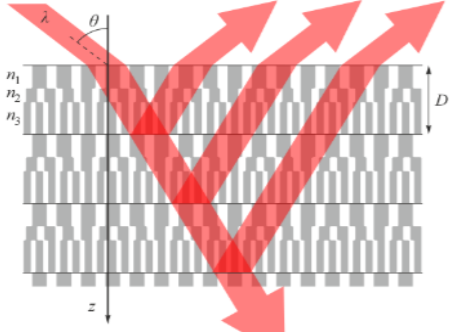
\includegraphics[scale=0.8]{2}
	\caption{Структура фотонного кристалла}
	\label{im:2}
\end{figure}

Рассмотрим параллельный монохроматический пучок с постоянной интенсивностью и длиной волны $\lambda$, падающий на фотонной кристалл. Пучки, отраженные от разных слоёв, интерферируют между собой. В результате интерференционная картина в отражённом свете имеет максимумы при определённых углах падения $\theta$ (минимумы пропускания наблюдаются при тех же углах), которые определяются условием:

\begin{equation}
2D\sqrt{n^2-\sin^2 \theta} = m\lambda
\label{eq:1}
\end{equation}
Где m=1, 2, … целые числа, означающие порядок интерференции.

Выражение (\ref{eq:1}) называется законом Брэгга-Снелла. Минимумы пропускания наблюдаются при тех же углах $\theta$. Если угол остается постоянным, а длина волны $\lambda$ изменяется, закон Брэгга-Снелла можно использовать, как уравнение для нахождения $\lambda$. 

С помощью угла дифракции можем выразить длину волны, которая соответствует минимуму пропускания: 
\begin{equation}
h\sin\phi = m\lambda
\label{eq:10}
\end{equation}
где $h = 1000$ нм -- период дифракционной решетки. Для нашего эксперимента $m=1$, объединяя (\ref{eq:1}) и (\ref{eq:10}), получим:

\begin{equation}
2D\sqrt{n^2-\sin^2 \theta} =h \sin\phi
\label{eq:11}
\end{equation}



Длины волн, удовлетворяющие закону Брегга-Снелла, будем называть длинами волн минимумов пропускания. Длины волн минимумов пропускания при $\theta=0$ нормальными длинами волн минимумов пропускания для данного фотонного кристалла.

\section{Выполнение работы}
\subsection{Часть 1}
\subsubsection{Ход работы}
\begin{enumerate}
\item Собрать экспериментальную установку.
\item Лампу поместить так, чтобы стоп-зону было хорошо видно, то есть поместить лампу на фокусном расстоянии.
\item Включить лампу, с помощью вращения дифракционного плеча найти первый дифракционный максимум.
\item При повороте фотонного кристалла, изменения угла падения можно увидеть, как по спектру движется темная полоска – минимум прохождения.
\item Изменяя угол падения и угол отражения, таким образом, чтобы середина стоп-зоны совпадала с черной отметкой дифракционной решётки, снять данные для рассматриваемого фотонного кристалла.
\item Проанализировать, полученные данные.
\end{enumerate}

\subsubsection{Стоп-зона при $\theta = 0$}
Кристалл X:\\
\begin{equation}
\phi = 45 \pm 0.5 ^\circ
\end{equation}

Кристалл Y:\\
\begin{equation}
\phi = 29.2\pm 0.5^\circ
\end{equation}

\subsubsection{График зависимости угла поворота образца от угла дифракции $\theta(\phi)$}
\begin{figure}[H]
	\centering
	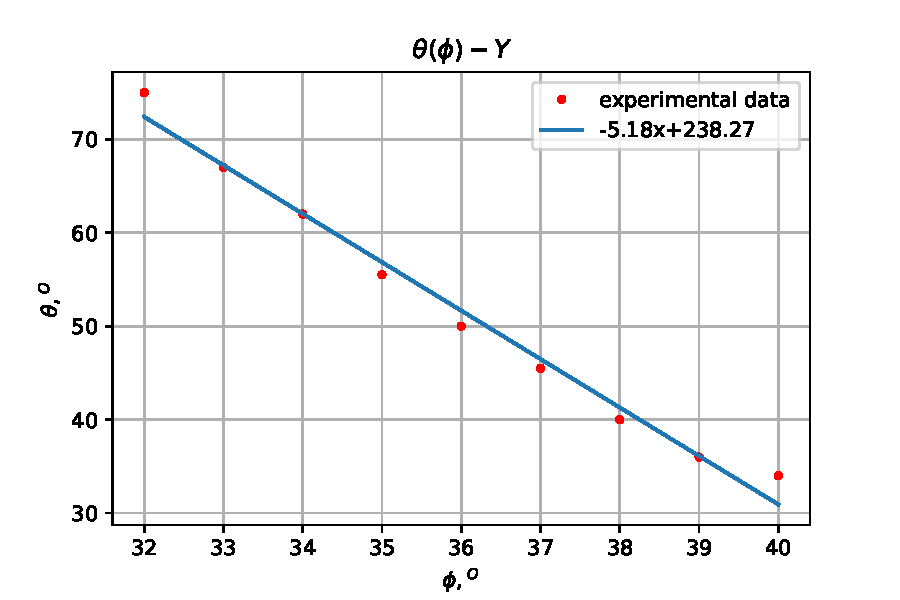
\includegraphics[scale=0.8]{Y_green_1}
	\caption{График линейной зависимости угла поворота образца от угла дифракции для Y}
	\label{im:6}
\end{figure}




\begin{figure}[H]
	\centering
	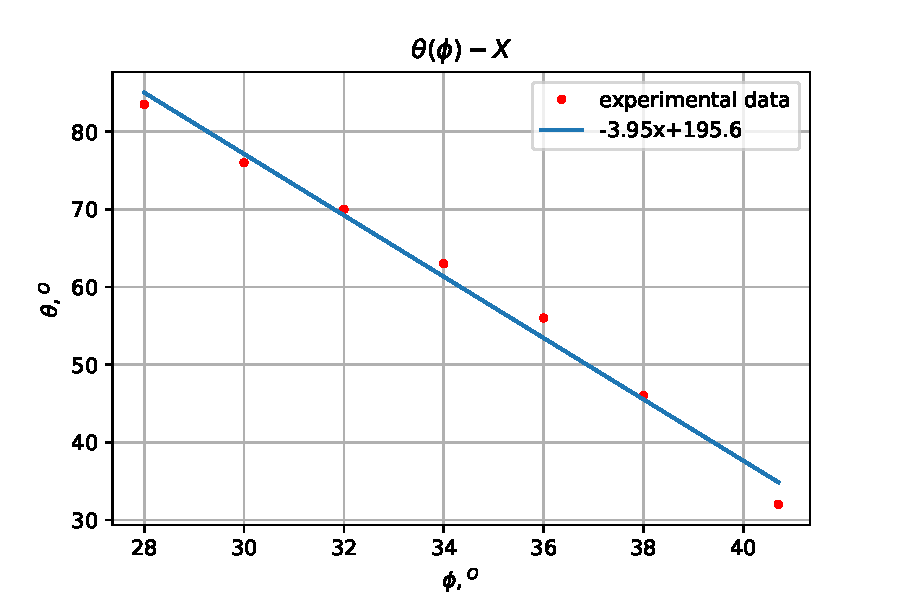
\includegraphics[scale=0.8]{X_red_1}
	\caption{График линейной зависимости угла поворота образца от угла дифракции для X}
	\label{im:7}
\end{figure}



\subsubsection{Средний показатель $n$ и $D$.}

Из (\ref{eq:11}) следует:
\begin{equation}
\sqrt{n^2-\left(\frac{h\sin\phi}{2D}\right)^2} =\sin\theta
\label{eq:2}
\end{equation}
Построим графики зависимости $\sin\theta(\sin\phi)$ -- для нахождения коэффициентов $n$ и $D$. Подгонка функцией (\ref{eq:2}) при помощи scipy дает следующие результаты:
\begin{figure}[H]
	\centering
	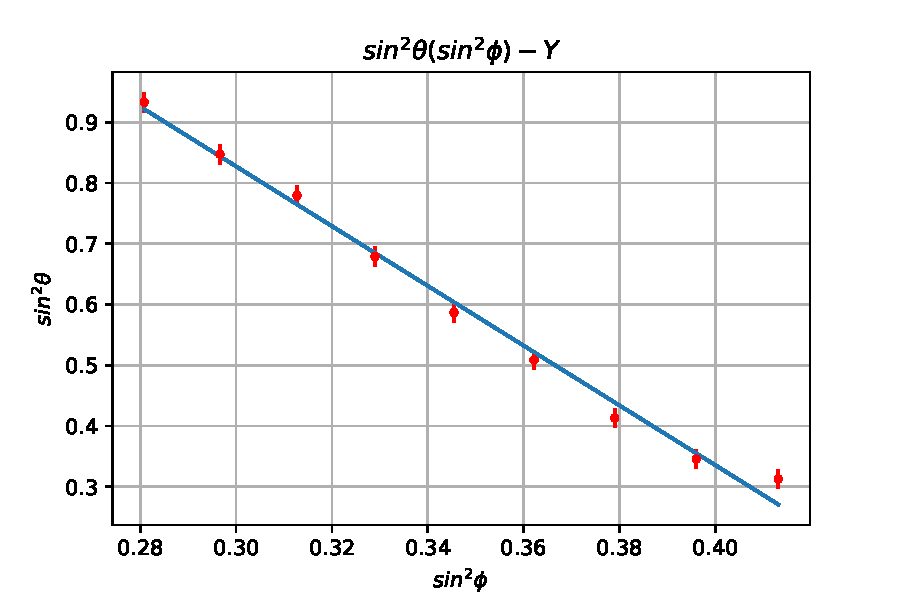
\includegraphics[scale=0.8]{Y_green_1_sin}
	\caption{График зависимости угла поворота образца от угла дифракции для Y}
	\label{im:10}
\end{figure}
 
\begin{equation}
n = 1.5\pm 0.01\;\;\;\;\;\;\; D = 225.5 \pm 2.2  \text{ нм}
\end{equation}


\begin{figure}[H]
	\centering
	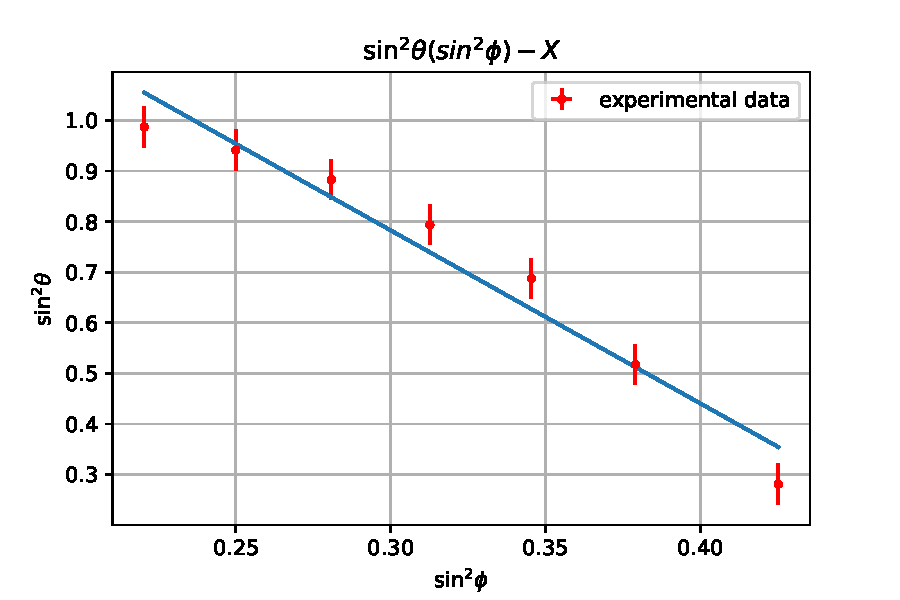
\includegraphics[scale=0.8]{X_red_1_sin}
	\caption{График зависимости угла поворота образца от угла дифракции для X}
	\label{im:11}
\end{figure}

\begin{equation}
n = 1.34\pm 0.04 \;\;\;\;\;\;\; D = 270 \pm 16 \text{ нм}
\end{equation}


\subsection{Часть 2}
\subsubsection{Ход работы}
\begin{enumerate}
\item Собрать установку с лазером ($\lambda_0$=660нм).
\item Повращать фотонный кристалл и заметить, что при изменении угла падения меняется значение тока, протекающего через мультиметр (интенсивности прошедшего света).
\item Поворачивая образец на разные значения $\theta$ снять данные тока с мультиметра.
\item Проанализировать полученные данные.
\end{enumerate}

\subsubsection{График зависимости интенсивности прошедшего лазерного излучения от угла $I(\theta)$}

\begin{figure}[H]
	\centering
	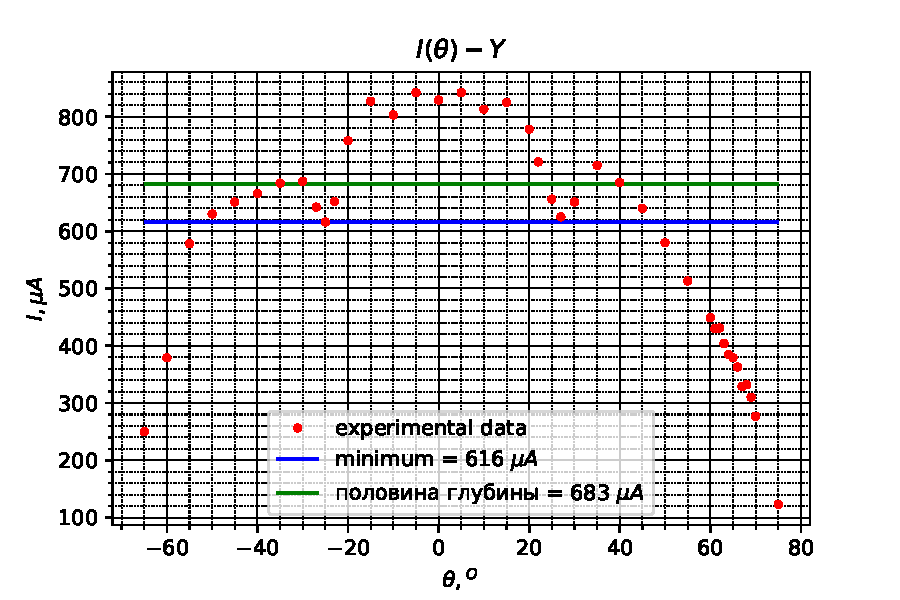
\includegraphics[scale=0.75]{Y_green_2}
	\caption{График зависимости интенсивности прошедшего лазерного излучения от угла для Y}
	\label{im:8}
\end{figure}
Значение минимума достигается при $\theta_0 =25\pm 0.5^\circ  $

Ширина провала: $19\pm 5^\circ $
\begin{figure}[H]
	\centering
	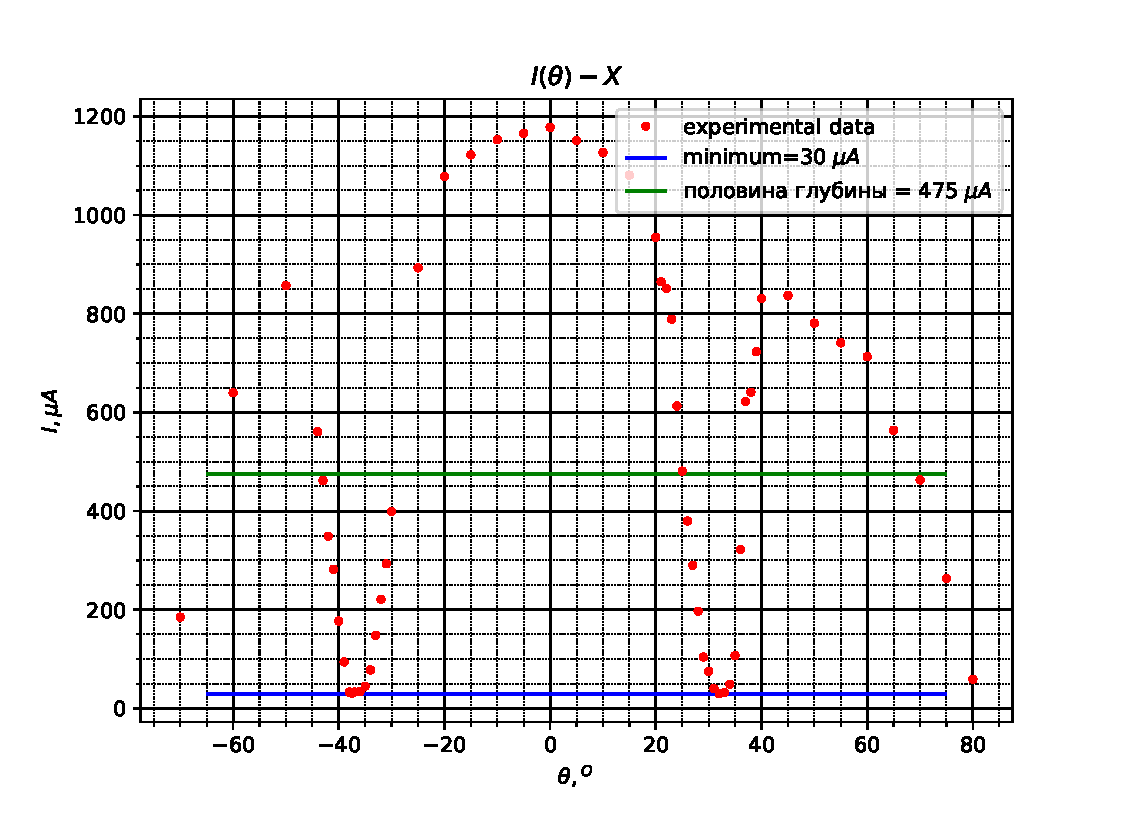
\includegraphics[scale=0.6]{X_red_2}
	\caption{График зависимости интенсивности прошедшего лазерного излучения от угла для X}
	\label{im:9}
\end{figure}
Значение минимума достигается при $\theta_0 =32\pm 0.5^\circ $

Ширина провала: $18\pm 5^\circ $
\subsubsection{Нормальная длина волны минимума пропускания $\lambda^{(n)}$}

Определим нормальную длину волны минимума пропускания:
\begin{equation}
\frac {n} {\sqrt{n^2 -\sin^2\theta_0}} = \frac{\lambda^{(n)}}{\lambda_0}\
\label{eq:3}
\end{equation}

Для образца Y:
\begin{equation}
\lambda^{(n)} = \frac {n\lambda_0} {\sqrt{n^2 -\sin^2\theta_0}} = 687 \pm1.5 \text{ нм}
\end{equation}

Для образца X:
\begin{equation}
\lambda^{(n)} = \frac {n\lambda_0} {\sqrt{n^2 -\sin^2\theta_0}} = 714.8  \pm 1.8 \text{ нм}
\end{equation}

Оценим разницу показателей преломления:
\begin{equation}
\frac {\Delta \lambda}{\lambda}=\frac{2\Delta n} {\pi n}
\end{equation}
\begin{equation}
\Delta n = \frac {\pi n\Delta \lambda}{2 \lambda}
\end{equation}

Для образца Y:

\begin{equation}
\Delta n = 0.09\pm0.01
\end{equation}

Для образца X:

\begin{equation}
\Delta n = 0.18\pm0.01
\end{equation}

\section{Вывод}

В ходе работы мы

\textbf{Пункт 1: Определение минимума прохождения}
	\begin{enumerate}
\item Определили, на какой длине волны находится стоп-зона при $\theta=0$.
\item  Измерили зависимость угла поворота образца $\theta$ от угла дифракции $\phi$.
\item  Построили линеаризованный график $\theta(\phi)$.
\item  Определили средний показатель преломления кристалла $n$ и период изменения показателя преломления $D$.
	\end{enumerate}

\textbf{Пункт 2: Зависимость интенсивности лазерного излучения от величины угла.}
	\begin{enumerate}
\item Измерили зависимость интенсивности лазерного излучения $I$ (в $\mu A$), прошедшего через фотонный кристалл, от величины угла $\theta$.
\item Построили график полученной зависимости.
\item Определили угол падения $\theta_0$, соответствующий минимуму пропускания на длине волны лазера.
\item Определили ширину провала $\Delta \theta_0$ на графике зависимости $I(\theta)$ на уровне половины его глубины.
\item Определили нормальную (при $\theta=0$ удовлетворяющую уравнению $2Dn=m\lambda^{(n)}$) длину волны минимума пропускания $\lambda^{(n)}$.
	\end{enumerate}
\end{document}